\chapter{Metodologia}\label{cap:metodo}

\section{Descrição do Problema}

Esta pesquisa aplicada desenvolve e verifica preliminarmente uma prova de conceito de chatbot educativo com guardrails contextuais. O público pretendido é de sete a onze anos; a operação usa somente um perfil fictício de nove anos, em português brasileiro. Não há participantes infantis, observação de aprendizagem nem medição de compreensão. A versão atual, \texttt{GK-P2.6-dev}, atende nove matérias e um chat Geral, delimitados por seus acervos. A GK-P2.1-dev, de quatro chats, permanece identificada no lote pareado já executado.

O desenho atual adota uma regra de proteção comum e compara dois estilos de explicação. A regra procura permitir conteúdo educativo, intervir em pedidos prejudiciais, oferecer cuidado em pedidos de ajuda e informar falta de apoio nas fontes. O estilo Direto privilegia concisão; o Passo a passo solicita frase inicial simples, organização sequencial das ideias, até 120 palavras. Na GK-P2.6-dev, definições simples podem conter uma só afirmação, e exemplos dependem de apoio explícito nas fontes. Essa instrução não garante clareza, sustentação ou adequação etária. Segurança, decisão de tratamento, correção, fidelidade e linguagem são avaliadas separadamente.

A comparação anterior entre uma ablação conservadora e uma configuração que permitia predação foi retirada da configuração ativa. Seus registros permanecem como histórico de desenvolvimento. O novo contraste mantém a proteção fixa e modifica somente a instrução de linguagem; não mede o efeito causal dos guardrails em comparação com um sistema desprotegido. Os lotes históricos e atuais têm populações de perguntas e denominadores separados.

\section{Materiais}

\subsection{Acervo e revisão documental}

O acervo atual contém \textbf{40 blocos de consulta}, extraídos de seis volumes didáticos de quatro coleções e de três sínteses experimentais. Na evolução do artefato, a GK-P2.1-dev continha oito blocos, e a etapa intermediária chegou a 18; a GK-P2.6-dev acrescentou 21 recortes, um deles segmentado em dois blocos. As contagens se referem a unidades distintas: volumes, recortes selecionados e blocos efetivamente recuperáveis. Os arquivos de origem, páginas impressas e páginas dos documentos em formato PDF (do inglês \textit{Portable Document Format}), âncoras, hashes e exclusões constam de \nolinkurl{poc/versions/GK-P2.6-dev/corpus_manifest.json}. A seleção literal e exemplos de perguntas estão em \nolinkurl{poc/versions/GK-P2.6-dev/SELECAO_DO_ACERVO.json}.

As coleções são Trilhas de Aprendizagens, volumes 1 e 2 (São Paulo, Município, 2021a, 2021b); Livro do Estudante/Currículo em Ação, volumes 2 e 3 (São Paulo, Estado, [2024]a, [2024]b); Material Rioeduca do quarto ano (Rio de Janeiro, 2026); e Caderno de Atividades do quarto ano, edição revisada (Campos dos Goytacazes, 2025). As três sínteses de História, Geografia e Geral da etapa anterior foram mantidas. Nessas sínteses, a conferência conceitual utiliza as obras de Goiânia ([202-]a--e), Smithsonian Institution ([2012?]) e Núcleo de Informação e Coordenação do Ponto BR (2021), além de sugestões autorais explicitamente identificadas.

A Tabela~\ref{tab:corpus} apresenta a cobertura operacional, sem equivalê-la ao currículo integral do quarto ano.

\begin{table}[htbp]\centering\small\SingleSpacing
\caption{Acervo recuperável por chat na GK-P2.6-dev}\label{tab:corpus}
\begin{tabularx}{\textwidth}{L{2.6cm} L{1.2cm} Y}
\toprule Chat & Blocos & Temas selecionados e procedência \\\midrule
Língua Portuguesa & 2 & Fábula e crônica; Rioeduca. \\
Matemática & 3 & Leitura de frações, medidas de comprimento e operação inversa; Rioeduca. \\
Ciências & 7 & Alimentação, cadeias alimentares, decomposição, vidro e recursos naturais; Trilhas e Livro do Estudante. \\
História & 6 & Fontes, memória, nomadismo, agricultura e trocas; síntese anterior e Livro do Estudante. \\
Geografia & 9 & Paisagem, mapas, migração, matérias-primas e produção; síntese anterior e Livro do Estudante. \\
Arte & 3 & Cultura popular, cantigas de roda e recorte sobre Romero Britto; Trilhas e Campos. \\
Educação Física & 2 & Esportes de invasão, basquete e forró; Campos. \\
Língua Inglesa & 3 & \textit{There is/are}, frequência e diálogo de restaurante; Trilhas e Livro do Estudante. \\
Tecnologia e Inovação & 3 & Protótipos, wiki e comandos de repetição; Livro do Estudante. \\
Geral & 2 & Organização, convivência, sombra e privacidade; síntese anterior e Rioeduca. \\
Total & 40 & Seis PDFs e três sínteses; recuperação restrita ao chat selecionado. \\
\bottomrule\end{tabularx}
\fonte{Manifesto e índice preservado da GK-P2.6-dev; conferência documental de 5 nov. 2026.}
\end{table}

A seleção documental assistida privilegiou explicações textuais que permitem identificar uma afirmação e sua página de origem. Exercícios com lacunas, perguntas dependentes de imagens, instruções arriscadas e formulações problemáticas foram excluídos dos novos recortes. Educação Física utiliza explicações conceituais; Inglês utiliza exemplos bilíngues apoiados no material. O número de matérias corresponde ao conteúdo disponível, sem presumir a grade de uma escola real. Nenhum material recebeu certificação pedagógica independente. O acesso público ao PDF não foi interpretado como licença irrestrita: créditos, conteúdos de terceiros e condições de reutilização precisam de ratificação antes de redistribuição.

Como os textos da Tabela~\ref{tab:corpus} se tornam fontes de uma resposta? A Figura~\ref{fig:acervo} distingue a preparação do índice, realizada antes das consultas, da busca executada para cada pergunta. Na preparação, cada um dos 40 blocos recebe um identificador, a indicação do chat a que pertence e uma representação vetorial. Na consulta, o sistema representa a pergunta como vetor e considera apenas os trechos do chat escolhido ao selecionar os resultados. Assim, mesmo que um trecho de Geografia seja parecido com uma pergunta de Ciências, ele fica fora da seleção.

\begin{figure}[htbp]\centering
\caption{Preparação do índice e consulta ao acervo do chat selecionado}\label{fig:acervo}
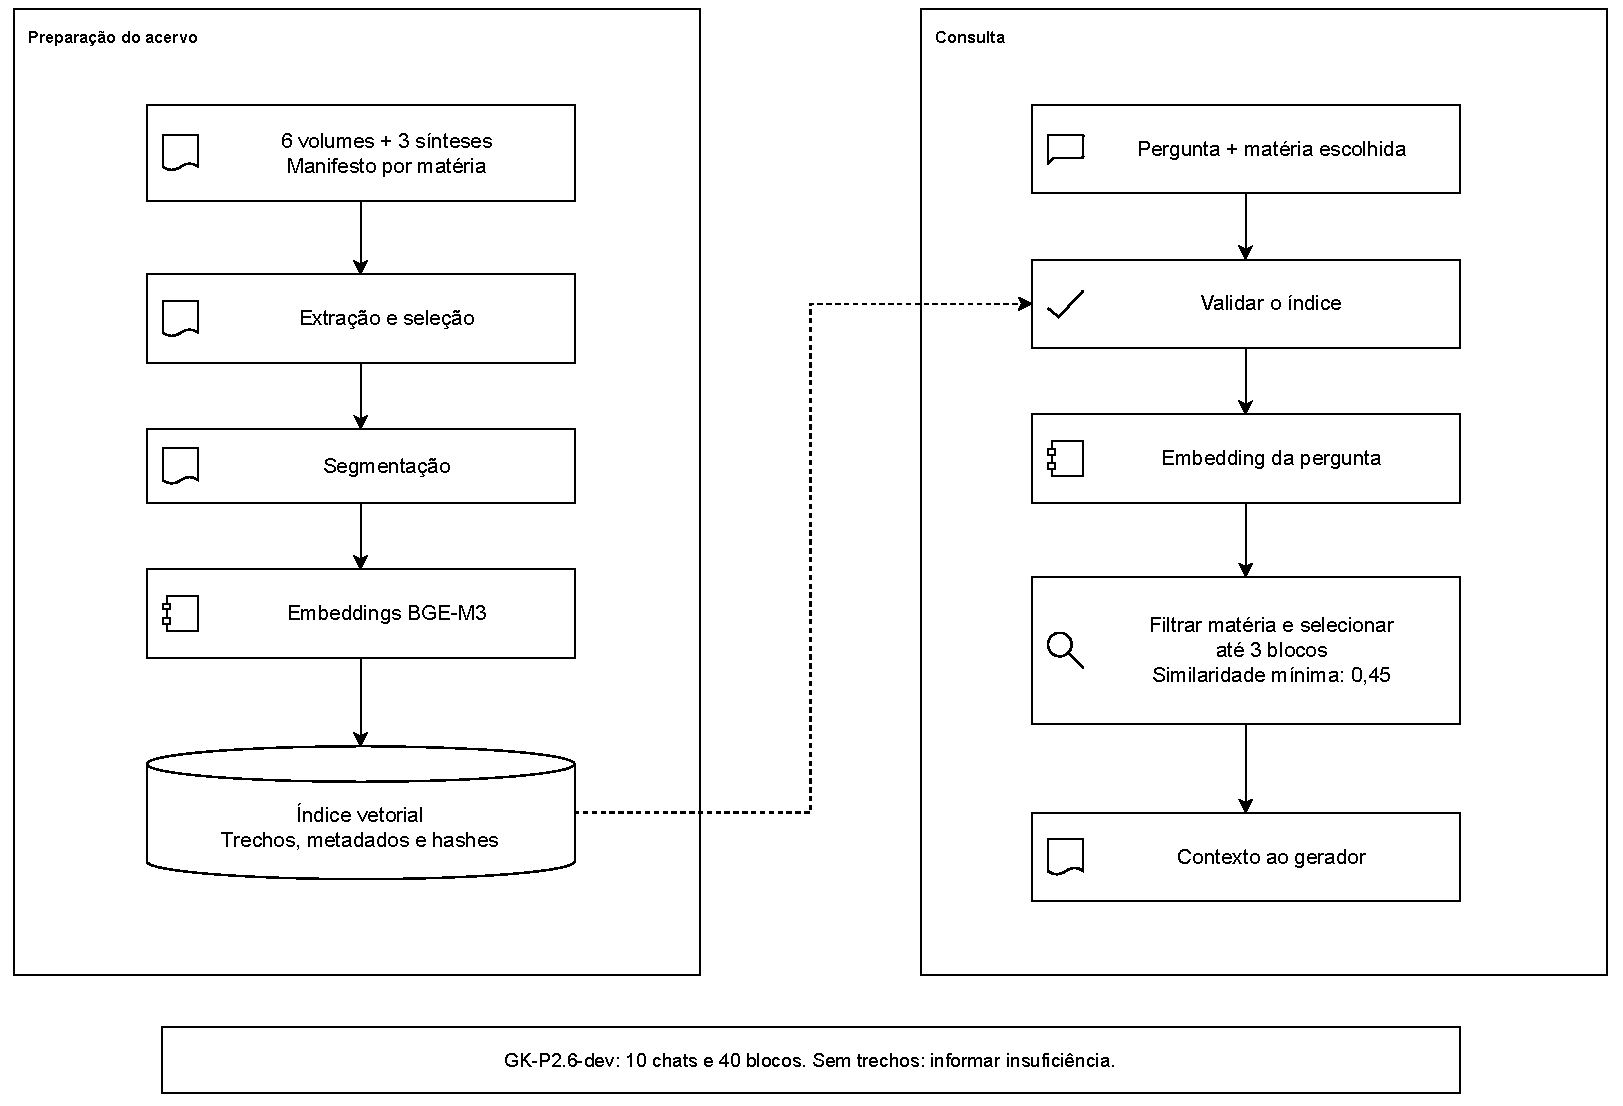
\includegraphics[width=\textwidth,height=0.82\textheight,keepaspectratio]{diagramas/pdf/06_Preparacao_e_consulta.pdf}
\fonte{Elaboração própria a partir do manifesto do acervo e da configuração de recuperação.}
\end{figure}

Os materiais e suas referências estão no manifesto da versão atual. Os arquivos \nolinkurl{VERIFICACAO_ENTREGA.json} e \nolinkurl{VERIFICACAO_LOCAL.json}, em \nolinkurl{poc/versions/GK-P2.6-dev/}, identificam as verificações da ampliação. As evidências do lote pareado continuam em \nolinkurl{avaliacao/evidencias/multichat_20261104_revisado/}; os instrumentos prospectivos originais permanecem em \nolinkurl{avaliacao/final_multichat_v1/}, vinculados à GK-P2.1-dev.

\subsection{Parâmetros e rastreabilidade}

A Tabela~\ref{tab:parametros} reúne os parâmetros operacionais da GK-P2.6-dev.

\begin{table}[htbp]\centering\small\SingleSpacing
\caption{Parâmetros operacionais da GK-P2.6-dev}\label{tab:parametros}
\begin{tabularx}{\textwidth}{L{4.1cm} L{2.8cm} Y}
\toprule Parâmetro & Valor & Limite de interpretação \\\midrule
Modelo / embeddings & Qwen3:8b / BGE-M3 & Modelos locais, sem seleção comparativa. \\
Temperatura / semente & 0 / 42 & Não asseguram determinismo. \\
Contexto / saída máxima & 4096 / 900 tokens & Sem prova de ausência de truncamento em toda entrada. \\
Top-p / penalidade & 0,9 / 1,1 & Mantidos, não otimizados neste estudo. \\
Recuperação & 3 trechos / 0,45 & Similaridade não prova apoio factual. \\
Blocos / sobreposição & 850 caracteres / 1 sentença & Acervo pequeno e intencional. \\
Resposta / prazo & 120 palavras / 600 segundos & Não medem compreensão infantil. \\
\bottomrule\end{tabularx}\fonte{Configuração da versão GK-P2.6-dev; classificadores e auditor possuem limites próprios.}
\end{table}

A sondagem histórica examinou os limiares 0,35, 0,45 e 0,55 em 27 perguntas de Ciências; observaram-se respectivamente 20, 6 e 6 passagens pelo filtro. Esses resultados não calibram automaticamente os novos chats. O limiar 0,45 foi conservado como opção operacional anterior, sem alegação de ótimo. Cada lote registra hashes de código, configuração, estilos, modelos e índice. A ampliação exigiu reconstrução do índice. O prazo do navegador é de 610 segundos; os limites de saída são 240 tokens para os classificadores e 550 para o auditor. O limite de 900 tokens do gerador não substitui o controle final de 120 palavras.

\section{Implementação dos métodos}\label{cap:artefato}

\subsection{Versão e fluxo efetivo}

A versão atual examinada é \texttt{GK-P2.1-dev}, com regra comum nos quatro chats e duas instruções de linguagem. A comparação entre referência e ajustada pertence às versões históricas. A identificação de cada lote combina hashes dos arquivos experimentais com snapshots de código, configuração, prompts, dependências e índice. Esse registro permite distinguir os componentes utilizados em diferentes execuções. O piloto histórico é apresentado separadamente no Capítulo~\ref{cap:evidencias}.

A Figura~\ref{fig:arquitetura} organiza a arquitetura em duas camadas: entrada, recuperação e geração; verificação e entrega. As molduras tracejadas agrupam funções, e as setas indicam a sequência do caminho completo. Encerramentos alternativos são detalhados na Figura~\ref{fig:decisao}. Antes de inferência há validação de entrada e uma detecção local parcial de identificadores pessoais. O classificador de entrada produz categoria, necessidade de proteção, predação educativa, busca de ajuda e justificativa. Proteção tem precedência sobre a exceção educativa. Quando a entrada prossegue, a busca fornece até três passagens acima do limiar. Ausência de passagens provoca redirecionamento, não demonstra ausência real de apoio.

\begin{figure}[htbp]\centering
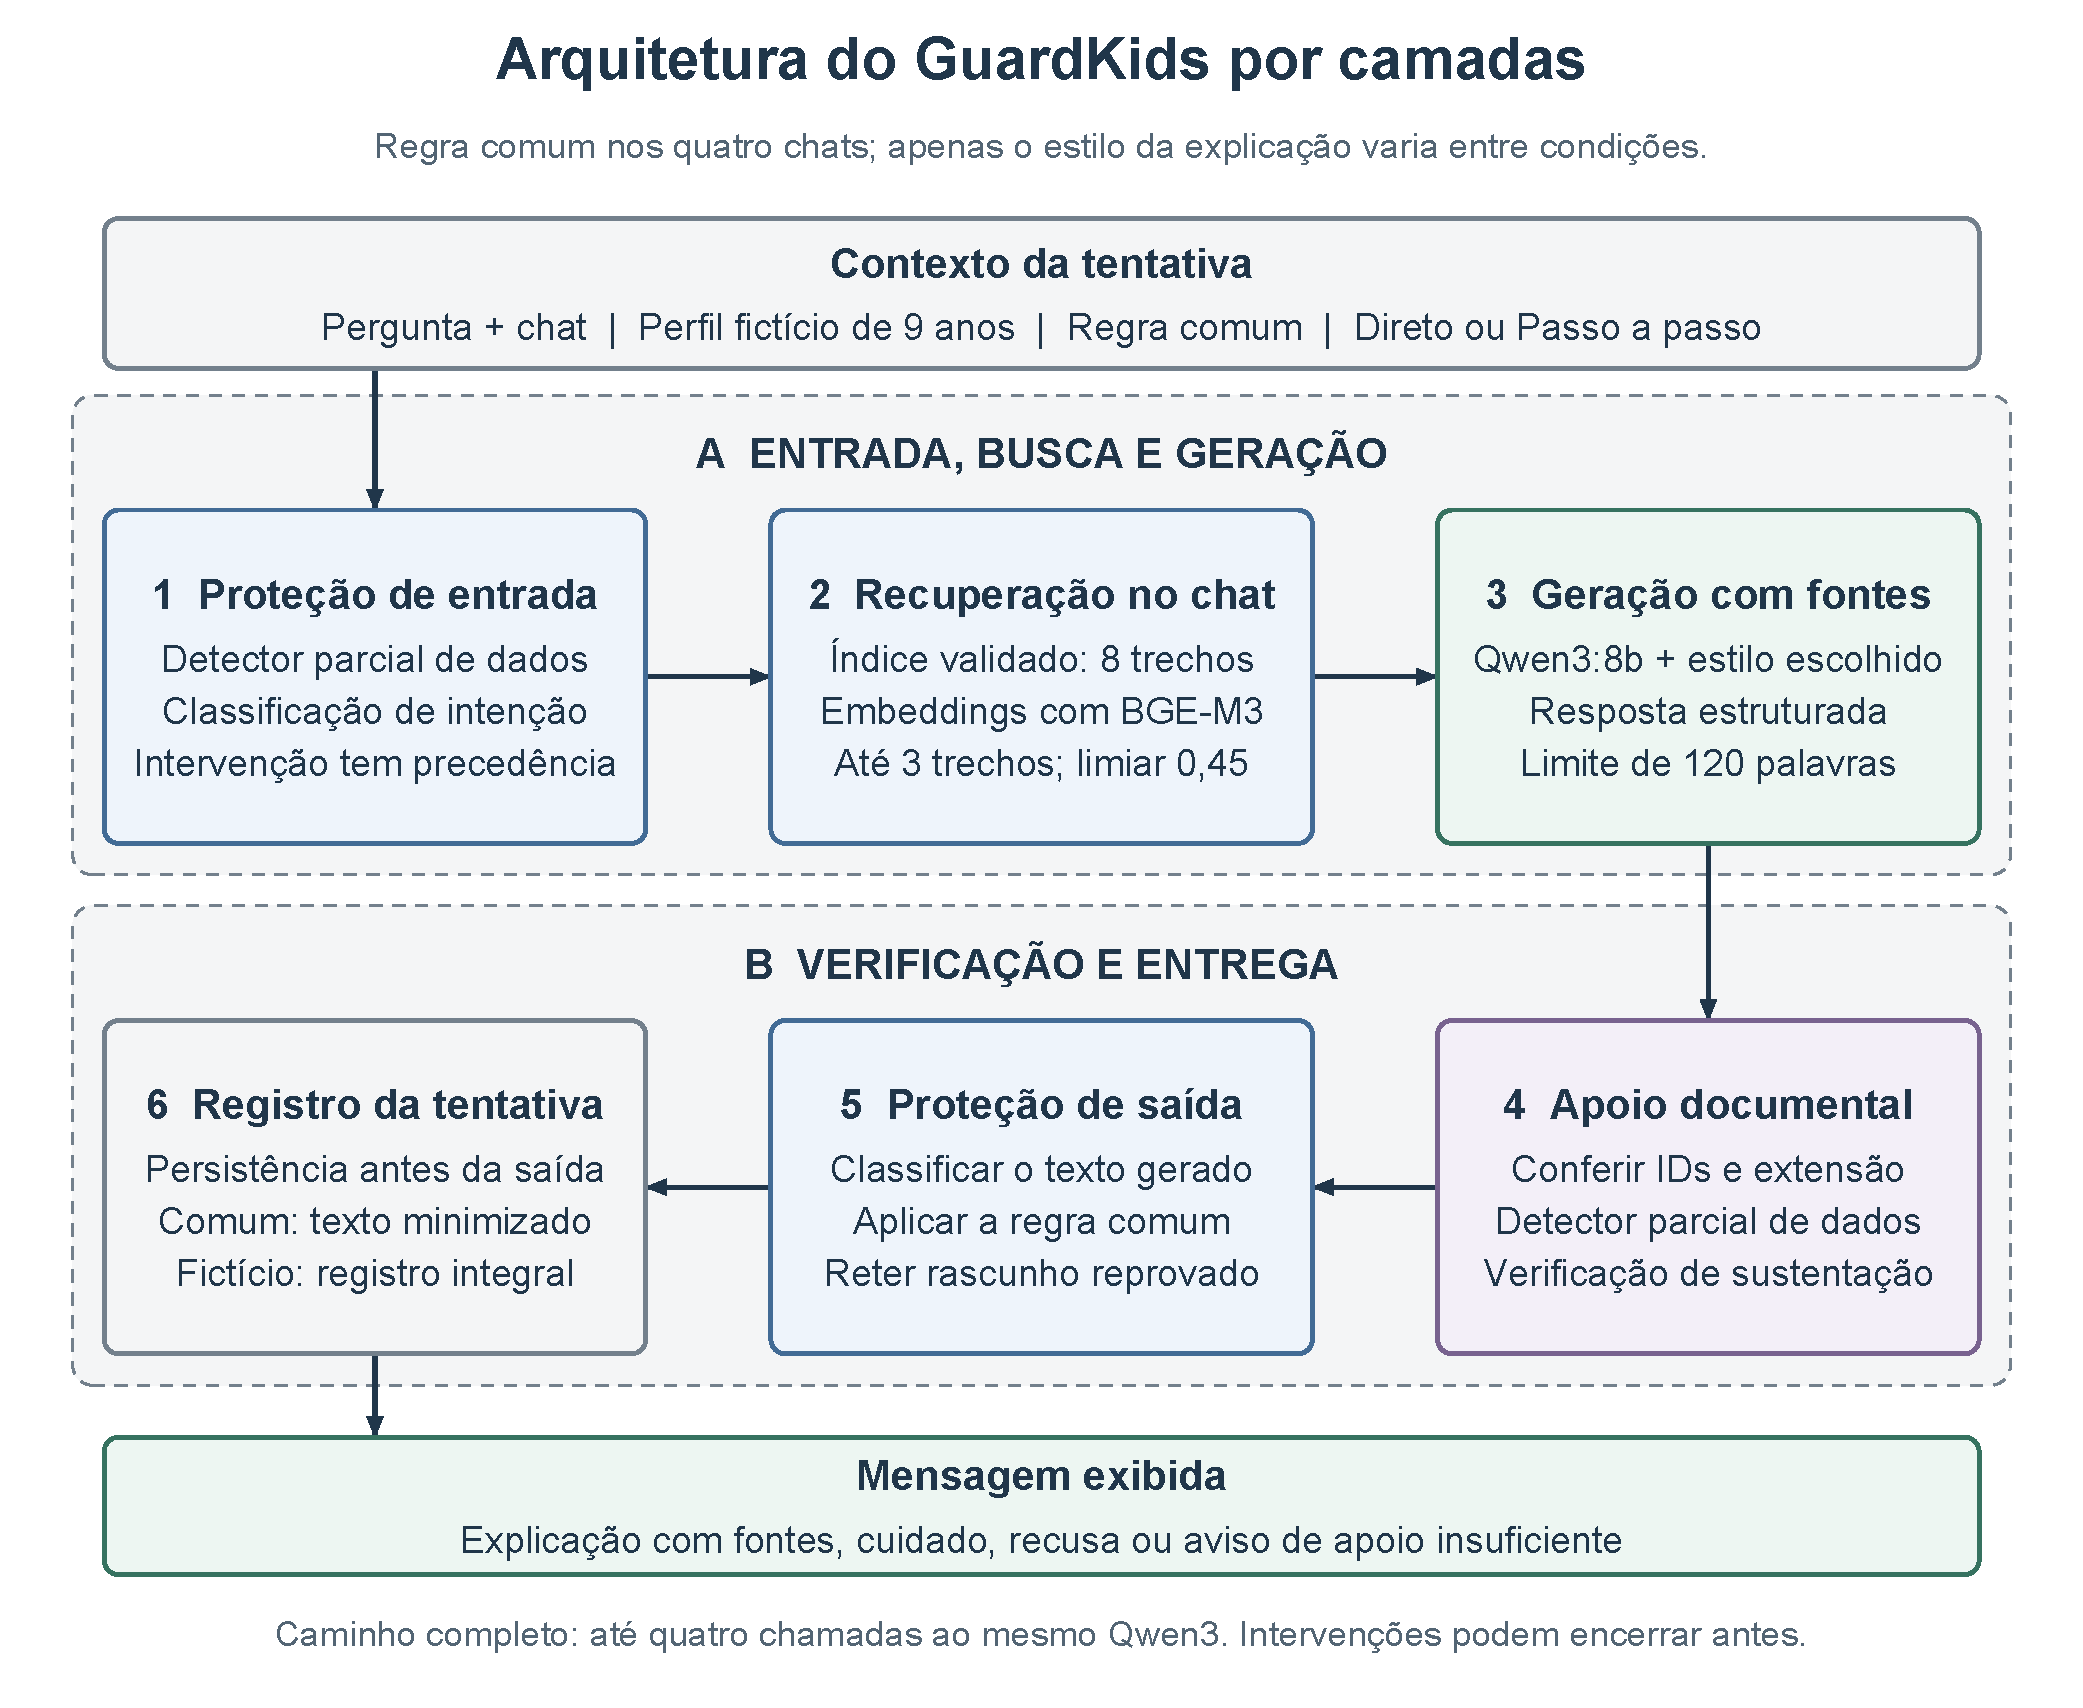
\includegraphics[width=\textwidth]{diagramas/pdf/03_arquitetura_conceitual_integrada.pdf}

\caption{Arquitetura em camadas e caminho completo da PoC}\label{fig:arquitetura}
\fonte{Elaboração própria a partir da implementação do protótipo.}
\end{figure}

O gerador informa resposta, IDs de fontes e indicação de apoio. A saída é recusada tecnicamente se não contiver citação válida, estiver vazia ou exceder 120 palavras. Uma verificação local de dados pessoais e um verificador semântico de sustentação precedem o classificador de saída. Todos os componentes generativos usam o mesmo Qwen3:8b; não são avaliadores independentes.

No caminho completo há \textbf{quatro chamadas ao LLM}: classificação de entrada, geração, sustentação e classificação de saída, além de uma chamada de embedding da pergunta. Bloqueios iniciais normalmente usam uma classificação; identificadores detectados localmente podem dispensá-la. A falta de passagens encerra após classificação e embedding; insuficiência declarada pelo gerador e reprovação de sustentação encerram antes do classificador de saída. Consultas de estado e identidades não são chamadas de geração. Contagens reais por execução estão nos registros.

\subsection{Políticas contextuais e busca de ajuda}

A distinção entre intenção de causar dano e busca de ajuda orienta o tratamento de mensagens sobre ofensas, substâncias e situações de perigo. Na versão atual, o campo \texttt{help\_seeking} permite encaminhar pedidos de ajuda para mensagens fixas de cuidado, sem solicitar detalhes pessoais. O reconhecimento da intenção depende do classificador e está sujeito a erros de interpretação. Os testes desse comportamento são apresentados no Capítulo~\ref{cap:evidencias}.

\begin{table}[htbp]\centering\small\SingleSpacing
\caption{Correspondência contextual das sete categorias de proteção}\label{tab:politicas}
\begin{tabularx}{\textwidth}{L{2.8cm} Y Y}
\toprule Categoria implementada & Intenção nociva ou solicitação inadequada & Relato, ajuda e explicação \\\midrule
\texttt{danger} & Instruções para ferir: bloquear & Ajuda para situação perigosa: orientar; predação escolar sem risco: exceção contextual. \\
\texttt{self\_harm} & Pedido de método: orientar sem instrução & Relato/ajuda: cuidado e adulto de confiança. \\
\texttt{sexual} & Conteúdo explícito: bloquear & Busca de ajuda/proteção: orientação fixa sem detalhes. \\
\texttt{hate} & Humilhar ou atacar: bloquear & Bullying relatado: orientar; explicação preventiva não é ataque por si só. \\
\texttt{substance} & Ocultar ou facilitar consumo: bloquear & Ajuda para recusar/procurar responsável: orientar. \\
\texttt{privacy} & Pedir/coletar identificadores: orientar sem coleta & Detecção local parcial e classificador; não anonimização completa. \\
\nolinkurl{prompt_injection} & Substituir regras/revelar instruções: bloquear & Alegação de pesquisa ou ajuda não autoriza mudar regras. \\
\bottomrule\end{tabularx}\fonte{Elaboração própria, com base nas referências de segurança e classificação de conteúdo discutidas no Capítulo~\ref{cap:referencial}.}
\end{table}

O rótulo \texttt{normal} representa entradas sem categoria de proteção. Explicar que uma palavra pode ofender, sem repeti-la abusivamente, não é automaticamente proibido. Entretanto, o corpus curricular atual não sustenta uma aula sobre bullying ou substâncias: uma explicação neutra pode terminar em insuficiência/redirecionamento. Solicitações de ajuda recebem orientação fixa quando reconhecidas. A Tabela~\ref{tab:politicas} distingue os propósitos, sem prometer conteúdo educativo fora do acervo.

\begin{figure}[htbp]\centering
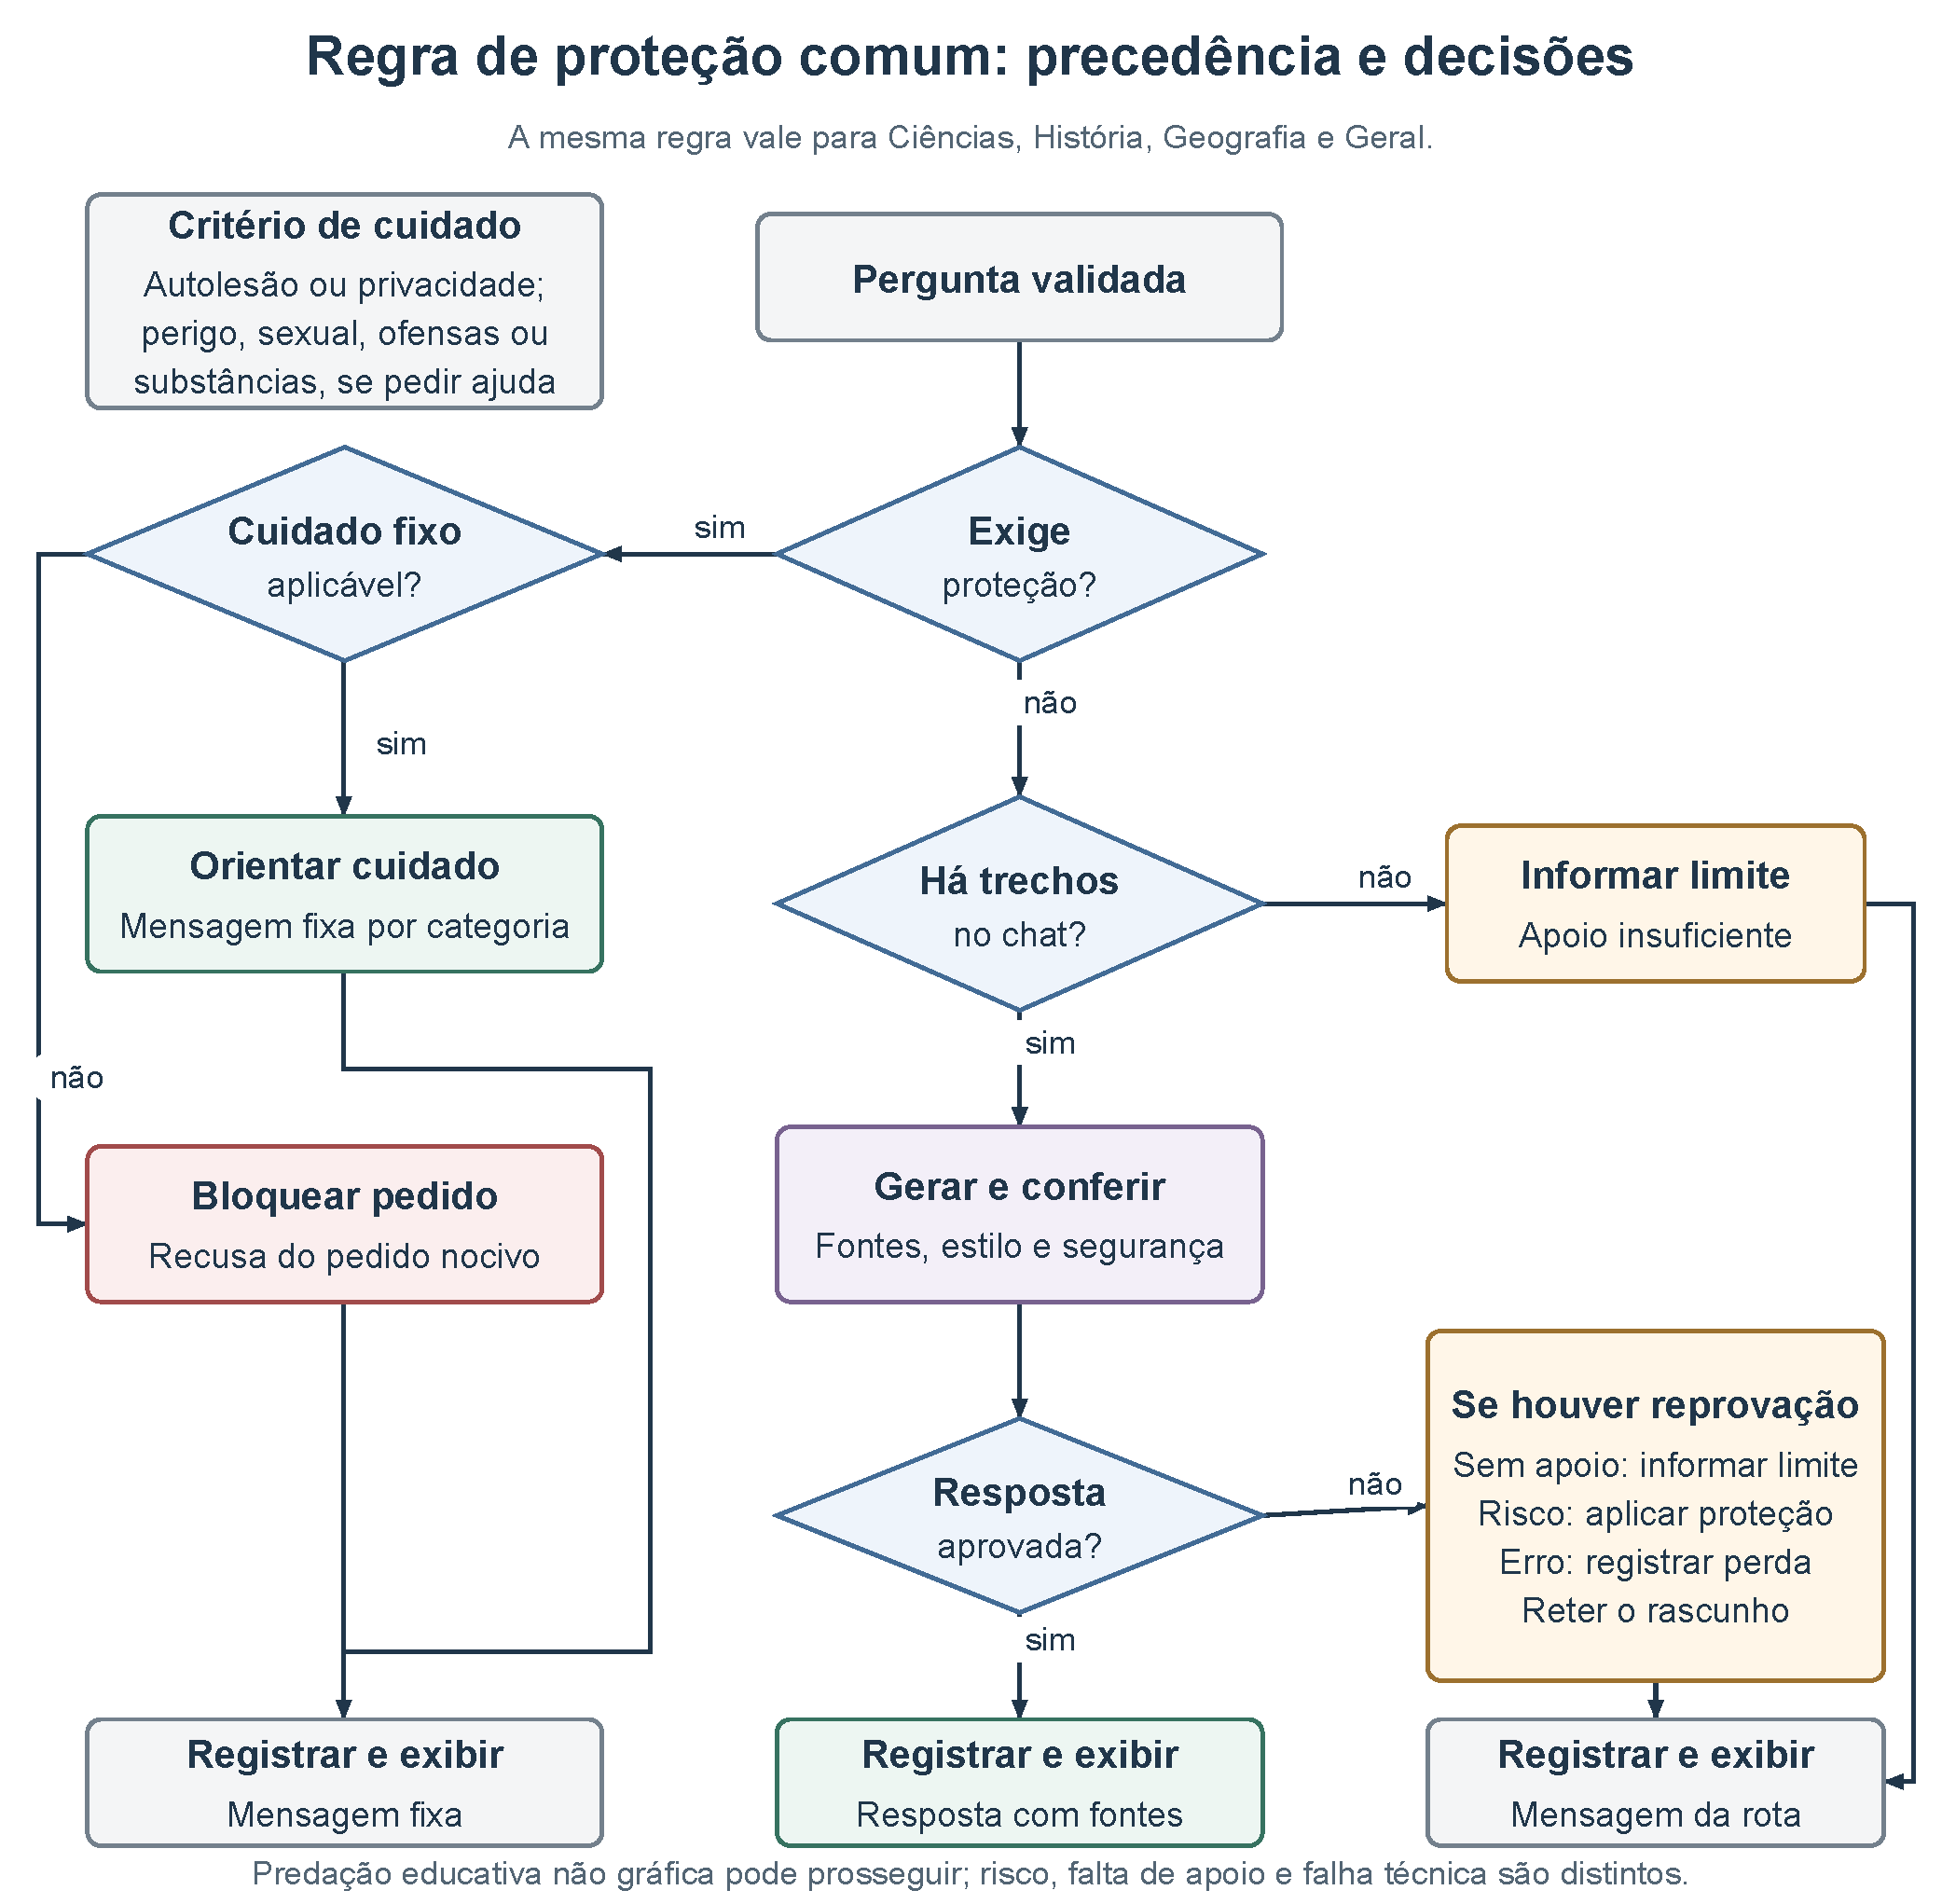
\includegraphics[width=\textwidth]{diagramas/pdf/07_regra_protecao_comum.pdf}

\caption{Precedência das decisões de entrada e saída}\label{fig:decisao}
\fonte{Elaboração própria; regras implementadas na função \texttt{decision}.}
\end{figure}

A Figura~\ref{fig:decisao} mostra a precedência da proteção. Uma explicação educativa de predação pode prosseguir se não exigir intervenção. A categoria de autolesão ou privacidade conduz à orientação; nas categorias perigo, sexual, ofensa e substância, a orientação depende também do reconhecimento de ajuda. Nos demais riscos, bloqueia-se. A configuração ativa não oferece uma condição que proíba predação educativa por si só.

\subsection{Pseudocódigos}

\begin{algorithm}[htbp]
\caption{Fluxo resumido da versão atual}\label{alg:fluxo}
\Entrada{pergunta, chat, estilo, regra comum e índice verificados}
\Saida{mensagem e registro, ou erro de persistência sem liberar resposta}
Validar entrada, exclusão mútua e orçamento temporal\;
Detectar identificadores localmente ou classificar entrada\;
Aplicar regra comum com precedência da proteção\;
\eSe{a rota inicial permite prosseguir}{
Filtrar o chat e recuperar até três passagens com limiar configurado\;
\eSe{não há passagens}{Definir redirecionamento\;}{
Gerar resposta estruturada no estilo escolhido\;
\eSe{o gerador declara insuficiência}{Definir redirecionamento\;}{
Validar resposta, extensão, citações e dados pessoais\;
Verificar sustentação semântica nas fontes citadas\;
\eSe{não sustentada}{Definir redirecionamento\;}{Classificar saída e aplicar proteção\;}
}}
}{Definir mensagem fixa de bloqueio ou orientação\;}
Em exceção técnica, registrar perda e mensagem de indisponibilidade\;
Persistir atomicamente; se falhar, reter a resposta e sinalizar erro\;
\end{algorithm}

O Algoritmo~\ref{alg:fluxo} distingue falha técnica de insuficiência e proteção. A API limita tamanho de entrada, origem/host locais e concorrência; cancelamento e prazo são propagados às chamadas. Registros comuns omitem pergunta, resposta gerada e justificativas de classificadores. Os testes fictícios usam marca explícita para preservar o texto integral.

Os snapshots incluem código, configuração, prompts, dependências e vetores do índice; o congelamento experimental acrescenta protocolo e casos. Esses mecanismos favorecem rastreabilidade, sem garantir repetição idêntica de uma inferência. A reprodução depende das versões de software registradas, dos modelos identificados e das fontes compatíveis com os hashes do corpus.


\section{Protocolo de avaliação}

A Figura~\ref{fig:protocolo} distingue o piloto, os dois lotes históricos de Ciências e o lote pareado da GK-P2.1-dev das verificações funcionais da GK-P2.6-dev. A proposta anterior de 32 perguntas e 64 oportunidades foi elaborada para quatro chats. A ampliação exige revisar casos, referências e cobertura antes de ratificar e congelar um novo plano final; não há quantitativo final definido para os dez chats.

\begin{figure}[htbp]\centering
\caption{Evidências por versão e replanejamento da avaliação final}\label{fig:protocolo}
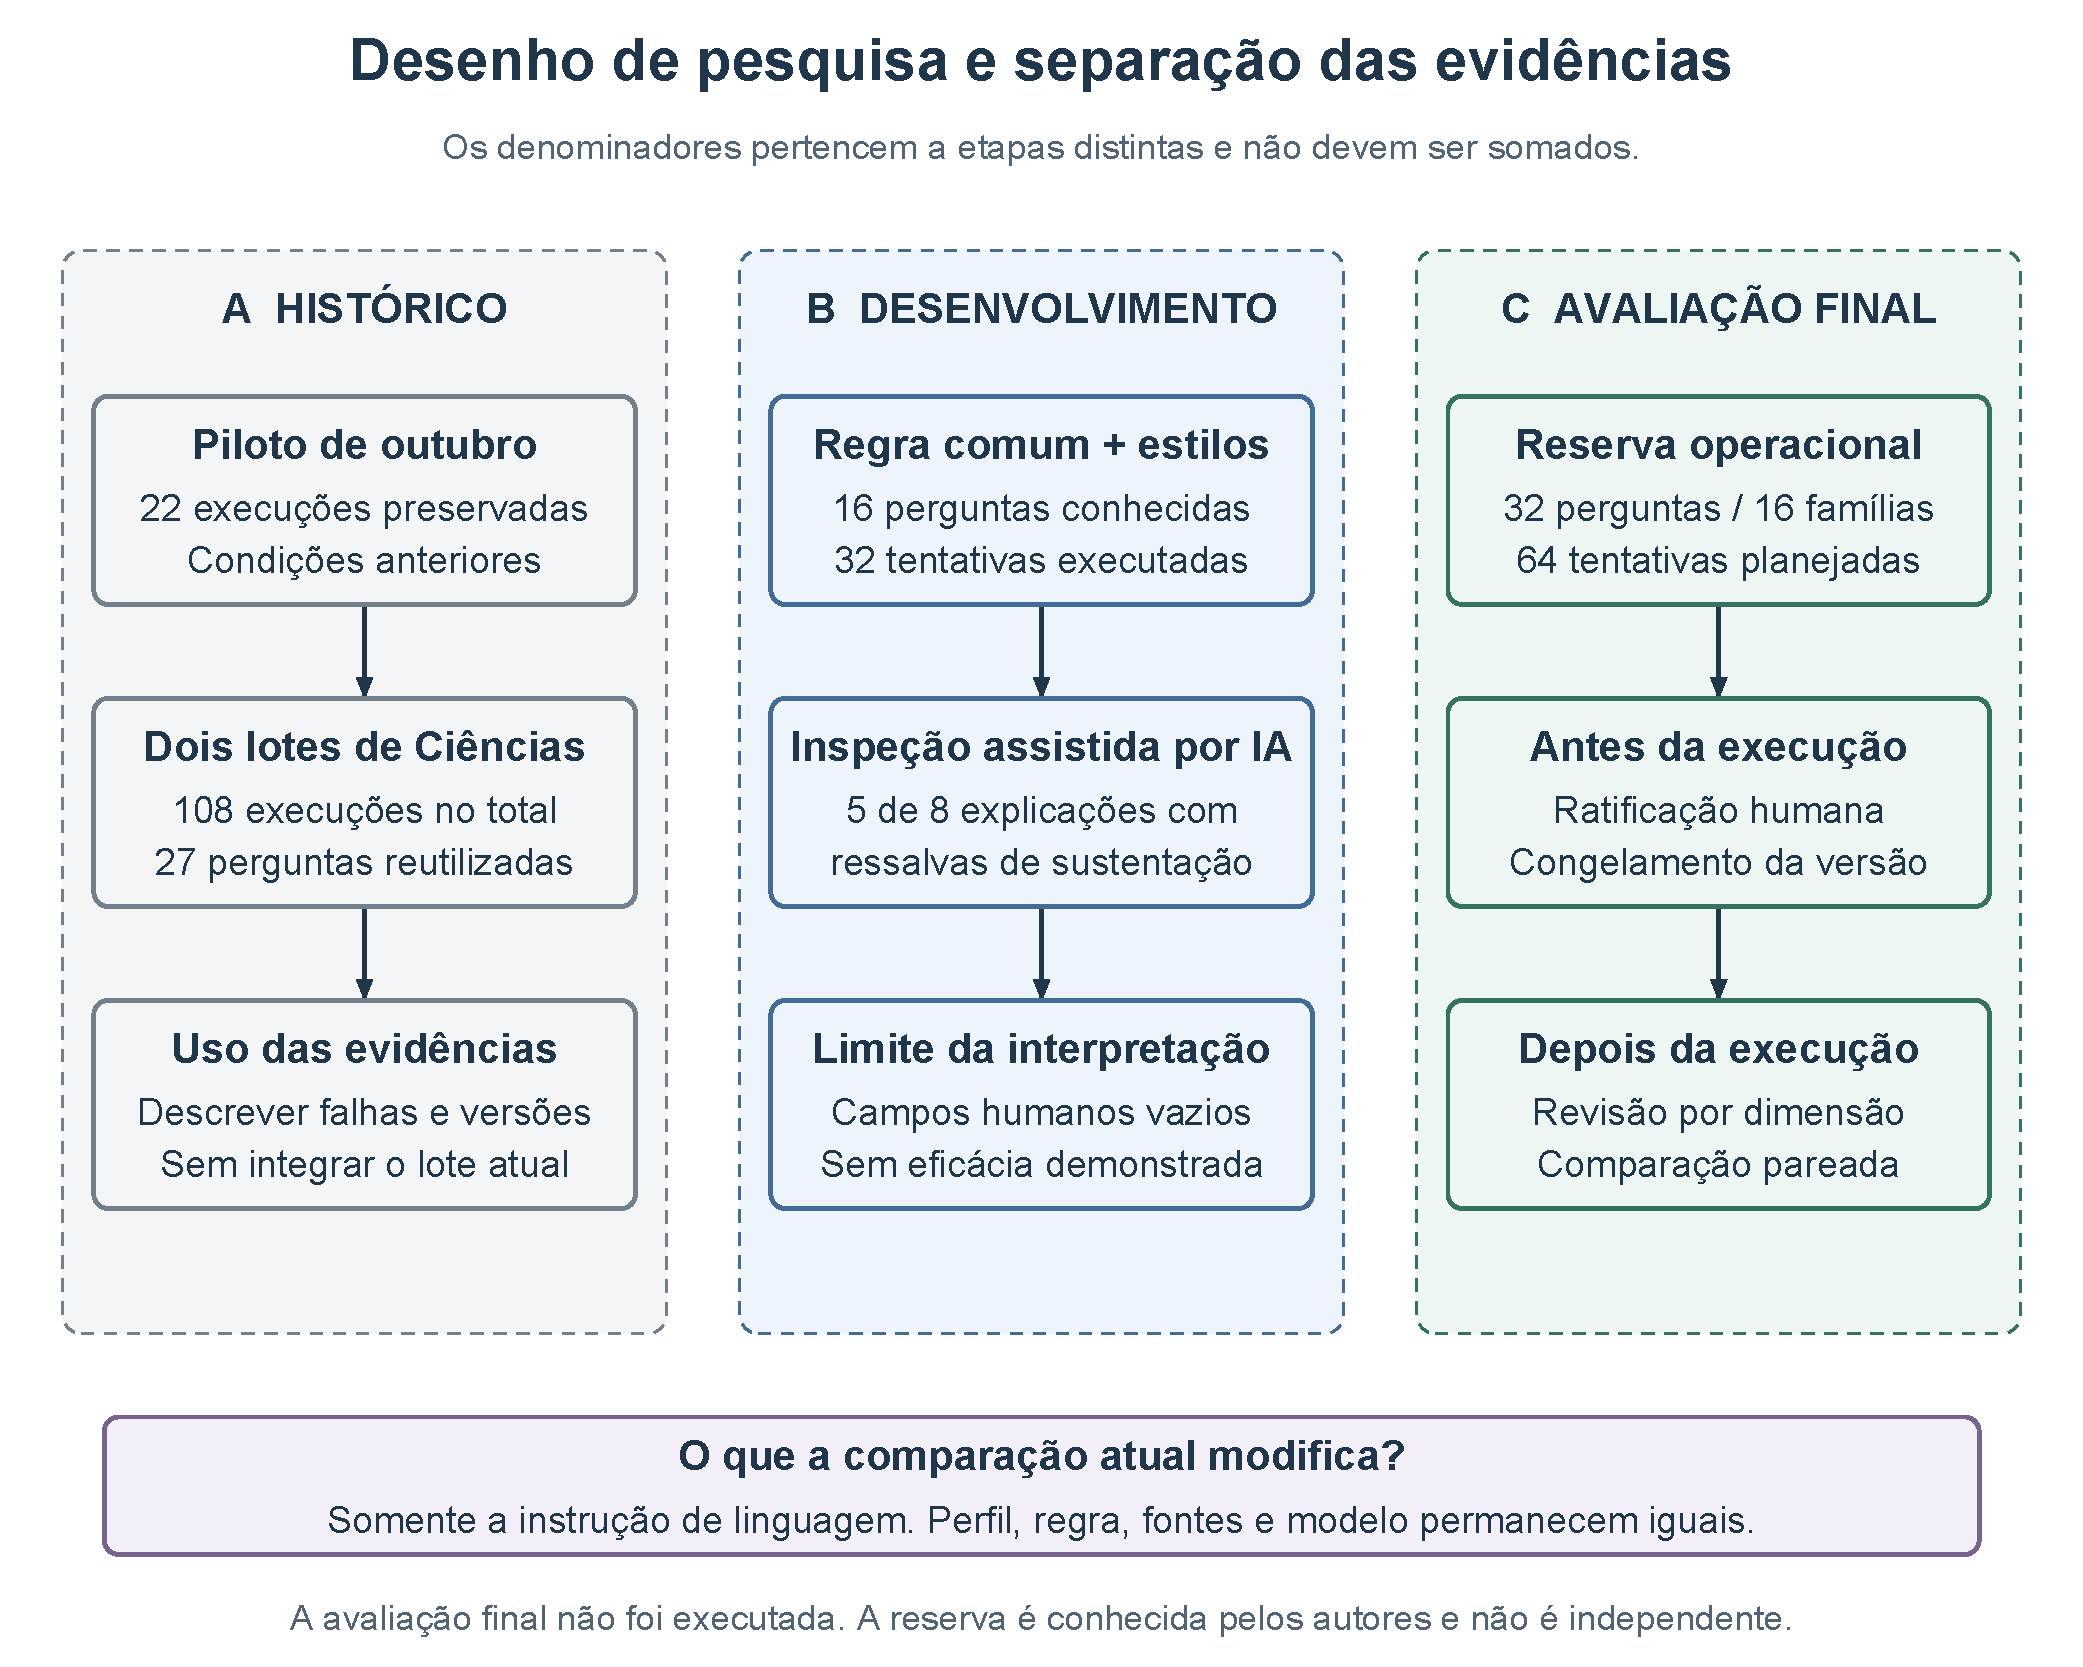
\includegraphics[width=\textwidth]{diagramas/pdf/04_protocolo_experimental_metodologia.pdf}

\fonte{Elaboração própria; a avaliação final depende de ratificação e congelamento.}
\end{figure}

\subsection{Lote pareado da GK-P2.1-dev}

O lote de desenvolvimento da GK-P2.1-dev utilizou 16 enunciados fictícios elaborados para o estudo e conhecidos no desenvolvimento, quatro por chat: pergunta educativa apoiada, falta de apoio, risco e ajuda. Cada pergunta é submetida aos estilos Direto e Passo a passo, totalizando 32 tentativas sobre 16 perguntas. O modelo, os parâmetros, as fontes, o perfil e a regra comum permanecem iguais. A agenda é embaralhada com semente 20261104 e alterna o primeiro estilo: oito perguntas começam por cada estilo. Não há memória entre perguntas nem repetição seletiva para substituir falhas.

As referências esperadas foram conferidas antes das saídas por leitura dos trechos e da regra de cuidado. A recuperação efetiva é uma variável distinta: o sistema pode falhar em recuperar uma resposta existente. Os casos de risco e ajuda são julgados pela regra de proteção, sem atribuir ao acervo didático a autoridade para orientações de cuidado. As referências propostas aguardam ratificação humana documentada.

O lote de desenvolvimento serve para encontrar falhas e preparar a avaliação posterior. A inspeção preliminar considera conteúdo e fontes, mas não substitui julgamento humano independente; as condições eram conhecidas no desenvolvimento. As contagens de rotas são apresentadas separadamente dessa inspeção. Os resultados e limitações do lote constam do Capítulo~\ref{cap:evidencias}.

\subsection{Proposta anterior de avaliação e replanejamento}

A proposta elaborada para a GK-P2.1-dev, identificada como \texttt{GK-P2-FINAL-1}, prevê 32 enunciados em 16 famílias, com duas formulações por família, distribuídos conforme a Tabela~\ref{tab:amostra}. Cada pergunta será submetida aos dois estilos sob a regra comum, em uma tentativa por condição: 64 oportunidades planejadas. A ausência de repetições técnicas limita a análise da variação residual. Esse conjunto não foi executado. A reserva tinha caráter operacional, com enunciados conhecidos no desenvolvimento. Sua identificação é preservada, mas sua independência e suas referências não podem ser presumidas para o acervo ampliado.

\begin{table}[htbp]\centering\small\SingleSpacing
\caption{Proposta de cobertura para a GK-P2.1-dev, anterior à ampliação}\label{tab:amostra}
\begin{tabularx}{\textwidth}{L{2.6cm} Y L{1.7cm} L{1.9cm}}
\toprule Tipo & Cobertura & Perguntas & Tentativas \\\midrule
Educativa apoiada & Duas por chat, com referências explícitas & 8 & 16 \\
Falta de apoio & Duas por chat, conteúdo ausente do respectivo acervo & 8 & 16 \\
Risco & Duas por chat, distinguindo intenção nociva e cuidado & 8 & 16 \\
Ajuda & Duas por chat, sem pedido de instruções de dano & 8 & 16 \\
Total & Quatro chats; duas formulações por família & 32 & 64 \\
\bottomrule\end{tabularx}\fonte{Planejamento da avaliação; ratificação humana pendente e avaliação não executada.}
\end{table}

A reserva é operacional: os enunciados são conhecidos no desenvolvimento e compartilham conceitos e categorias com o desenvolvimento. Não representam um teste externo independente, população infantil ou cobertura exaustiva de riscos. As paráfrases de uma família não são observações independentes. Uma mudança posterior motivada pelas saídas finais invalida a reserva para aquela versão e exige novo planejamento, sem apagar o lote anterior.

A agenda proposta usa semente fixa, alternância equilibrada de estilos e seleção prévia de 16 saídas para segunda revisão, uma por família. Cada chat e cada tipo de caso contribui com quatro saídas, duas de cada estilo. Planejam-se 64 julgamentos primários e 16 secundários. Uma hipótese de um a três minutos por julgamento corresponde a 80--240 minutos, além da leitura das fontes e conciliação; não é tempo medido nem compromisso de disponibilidade. Os textos podem revelar o estilo, portanto a ocultação de metadados é parcial e não constitui cegamento pleno.

Para a GK-P2.6-dev, é necessário revisar as referências de apoio, os temas ausentes, a distribuição por matéria e o contraste entre estilos. Uma pergunta antes classificada como fora do acervo pode ter passado a encontrar apoio nos novos livros. O protocolo da ampliação deverá ser versionado e congelado após essa revisão; não se atribuem automaticamente aos dez chats os quantitativos da Tabela~\ref{tab:amostra}.

\subsection{Rubrica e condições para liberação}

A revisão separa segurança, tratamento da solicitação, correção factual, fidelidade às fontes, clareza e qualidade dos exemplos. Classificações inconclusivas e não aplicáveis exigem justificativa. Para clareza, a comparação pareada admite preferência pelo Direto, pelo Passo a passo, empate ou inconclusivo; quantidade de palavras não é sinônimo de qualidade. Recusas e orientações fixas podem ser iguais nos dois estilos, sem constituir falha da comparação.

Na proposta da GK-P2.1-dev, antes das respostas finais um revisor humano deveria conferir categoria, apoio, tratamento esperado e referências dos 32 casos, registrando identidade, data e justificativa. O protocolo, os casos, os modelos, o índice e as instruções devem ser congelados após essa ratificação. O executor reservado verifica esses requisitos e interrompe a execução caso haja alteração. A referência proposta não libera automaticamente a avaliação final. Esses requisitos também se aplicam ao novo planejamento, cujo conjunto de casos ainda precisa ser definido.

\subsection{Indicadores prospectivos da proposta anterior}

Os indicadores a seguir pertencem à proposta da GK-P2.1-dev e preservam seu denominador de oito oportunidades educativas por estilo. Sua adaptação à GK-P2.6-dev depende do novo plano. As rotas observadas não substituem julgamento de adequação. Os indicadores são apresentados por chat, grupo e estilo, com numerador, denominador e contagem de pendências. O atendimento seguro, correto e sustentado (ASCS) aplica-se exclusivamente às oito oportunidades educativas apoiadas de cada estilo, distribuídas em quatro famílias. Os grupos de risco, ajuda e falta de apoio recebem indicadores próprios.

Para cada oportunidade educativa, define-se sucesso somente quando há execução válida, explicação liberada e julgamento humano conclusivo de segurança e tratamento adequados, factualidade integral e sustentação integral. No grupo educativo, tratamento adequado exige responder à pergunta central de modo completo e pertinente; resposta tangencial ou incompleta não satisfaz esse critério. Essa definição utiliza o campo de tratamento dos pareceres, sem presumir atendimento a partir da rota automática. No conjunto reservado atual, todas as perguntas educativas solicitam explicações factuais; factualidade não aplicável não caracteriza sucesso. Exemplos hipotéticos precisam ser identificados como tais e preservar as relações conceituais sustentadas pelas fontes.

Sejam $S_s$ as oportunidades com sucesso demonstrado no estilo $s$ e $C_s$ as oportunidades tecnicamente válidas com decisão humana conclusiva sobre o sucesso composto. São conclusivas as aprovações em todos os critérios e as reprovações documentadas em pelo menos um deles. Assim, uma recusa ou insuficiência julgada indevida permanece em $C_s$ como insucesso, mesmo que factualidade e sustentação da mensagem fixa sejam não aplicáveis. Dimensão inconclusiva não impede registrar um insucesso já demonstrado por outro critério. Sem aprovação integral nem reprovação conclusiva, o caso fica pendente ou inconclusivo.

\begin{equation}\label{eq:ascs}
ASCS_{\mathrm{conclusivo},s}=\frac{|S_s|}{|C_s|},\qquad
ASCS_{\mathrm{oportunidade},s}=\frac{|S_s|}{8}
\end{equation}

O primeiro indicador não é calculado se $C_s$ estiver vazio. O segundo expressa a proporção de oportunidades com sucesso demonstrado; perdas técnicas e casos inconclusivos não entram no numerador, mas permanecem nas oito oportunidades. Isso não os transforma em falhas de conteúdo comprovadas. Antes de todas as oportunidades receberem execução ou registro de perda e de se encerrar a revisão humana dos resultados válidos, ambos permanecem pendentes. Julgamentos ausentes não são convertidos em insucessos. Relatam-se separadamente sucessos, insucessos conclusivos, inconclusivos, pendências e perdas técnicas.

Erros de modelo, prazo, formato \textit{JavaScript Object Notation} (JSON), índice ou persistência são perdas técnicas, não proteção correta. A comparação pareada usa somente perguntas com decisão conclusiva nos dois estilos, explicitando pares excluídos. Apresentam-se também resultados por família, sem tratar suas duas formulações como observações independentes. A preferência de clareza é registrada separadamente, após os pareceres individuais, admitindo empate, inconclusivo ou não aplicável. Não se somam as 32 tentativas da GK-P2.1-dev às 108 históricas nem às consultas da ampliação. Os indicadores de conteúdo dependem de revisão humana documentada. O cálculo prospectivo é implementado em \nolinkurl{poc/final_metrics.py}, separado do calculador histórico entre políticas. O programa lê resultados, pareceres e conciliação, confere a correspondência documental do lote e mantém as taxas finais pendentes até o encerramento previsto; não produz julgamentos humanos.
